\section{The Higgs Mechanism and Electroweak Symmetry Breaking}
\label{sec:higgs_description}

The missing mass-terms for the fields in \SML~are provided by the
Brout-Englert-Higgs (BEH) mechanism~\cite{Englert:1964et,Higgs:1964ia,Higgs:1964pj}.
Before describing the specifics of the BEH mechanism, we should first describe the problem
of why \SML~doesn't support general mass terms for any of the fields in the first place.
That is, for example, why can't a fermion term like $m \bar{f} f$ exist in \SML?

Adding mass terms to \SML~for the fermions explicitly breaks the underlying \SUtwo~
gauge symmetry. This can be understood if we recognize the experimentally supported
fact that the left-handed fermions appear as \SUtwo~doublets and that the
right-handed fermions as singlets,
\begin{align}
	m\bar{f}f &= m \bar{f}(P_L + P_R)f \notag \\
				   &= m \bar{f} P_L P_L f + m \bar{f} P_R P_R f  	\label{eq:bad_fermion_mass_term}\\
				   &= m \left( \bar{f}_R f_L + \bar{f}_L f_R \right), \notag
\end{align}
where we have used identity relations of the projection operators $P_L$ and $P_R$ and the fact that $\bar{f}P_L = \bar{f}_R$ (and vice-versa). The last line of Equation~\ref{eq:bad_fermion_mass_term} involve terms
mixing \SUtwo~doublets with \SUtwo~singlets. Such a term is therefore not allowed if we wish to keep the \SUtwo~gauge symmetry intact.

Mass terms for the gauge bosons, of the form $m B_{\mu} B^{\mu}$, also do not work. For the Abelian \Uone~symmetry, for example, gauge invariance implies invariance of \SML~under transformations
of the form $B_{\mu}^{\prime} \rightarrow B_{\mu} - \partial_{\mu}\chi /g$. Such a mass term for
the gauge bosons is clearly not invariant under such a transformation. Even forgoing this fact,
adding such a term would quickly lead to non-renormalizable divergences appearing in the theory,
due to the longitudinal field components that appear in massive field propagators, rendering \SML~meaningless.

The BEH mechanism provides a way out of this problem. It refers to the introduction of a
spin-0 field, the Higgs field (Table \ref{tab:sm_content}), to the SM along with its corresponding interaction
terms to \SML: the last three terms of Equation~\ref{eq:sm_lagrangian}. The final two terms make up
what is referred to as the Higgs potential and can be expressed as,
\begin{align}
	V(\phi) = - \mu^2 \phi^2 - \lambda \phi^4
	\label{eq:higgs_potential}
\end{align}
The Higgs field is an \SUtwo~doublet and it can be seen that the interactions
described by Equation~\ref{eq:higgs_potential} respect \SUtwo~gauge symmetry.
If $\mu^2>0$, nothing all too interesting occurs and Equation~\ref{eq:higgs_potential} describes
a self-interacting, complex scalar field. If we take $\mu^2<0$, however, then the classical
potential described by Equation~\ref{eq:higgs_potential} has non-zero minima located at
$\phi = \pm v$ with $v = \sqrt{-\mu^2 / \lambda}$.
This is illustrated in Figure~\ref{fig:higgs_ewsb}. We see that the stable equilibrium point $\phi_0$
of the Higgs potential, the \textit{Higgs vacuum expectatin value} (vev), is not at $\phi = 0$
but at $v$,
\begin{align}
	\phi_0 = \frac{1}{\sqrt{2}} \left( \begin{matrix} 0 \\ v \end{matrix} \right)
	\label{eq:higgs_vev}
\end{align}
The choice of Equation~\ref{eq:higgs_vev} to represent the Higgs vacuum is motivated by
the requirement that the vacuum not be electrically charged --- a fact motivated very much
by experiment and everyday experience --- so the up-type \SUtwo~component of the Higgs field, $\phi^+$ (Table \ref{tab:sm_content}), is chosen to be zero for $\phi_0$. The choice of an
electrically neutral vacuum sets the rest of the \SUewk~structure of the complex Higgs field
since, by the Gell-Mann-Nishijima relation (Equation~\ref{eq:gell_mann_nishijima}) and charge
conservation,
a  neutral \SUewk~field should have down-type \SUtwo~quantum numbers and \Uone~hypercharge
$Y=1$,
\begin{align}
	Q = T_3 + \frac{1}{2}Y \rightarrow Q_{\phi_0} = -\frac{1}{2} + \frac{1}{2} \times 1 = 0.
	\label{eq:higgs_charge}
\end{align}

Note that Equation~\ref{eq:higgs_vev} states that only one component of the Higgs \SUtwo~doublet
attains a non-zero vev. This clearly means that the \SUtwo~gauge symmetry is not respected
by the choice of $\mu^2 < 0$ and that the electroweak \SUewk~symmetry is
\textit{spontaneously broken}.\footnote{A symmetry of a Lagrangian is said to be
	`spontaneously' broken if the Lagrangian of the underlying theory
	respects the symmetry but it gets broken through dynamical means or if the lowest-energy
	state (vacuum) does not respect the symmetry.
} The Higgs field
acquiring a non-zero vev is then referred to as the \textit{electroweak symmetry breaking} (EWSB) of the SM.

To further examine the physical consequences of EWSB,
we perturb the Higgs field about its minimum value,
\begin{align}
	\phi(x) \propto \left( \begin{matrix} 0 \\ \frac{1}{2}(v + h(x)) \end{matrix} \right),
	\label{eq:higgs_perturb}
\end{align}
where $h(x)$ correspond to excitations of the Higgs field that represent the physically observable
Higgs boson.
Inserting Equation~\ref{eq:higgs_perturb} into the $\mathit{D}_{\mu}\phi$ terms
of Equation~\ref{eq:sm_lagrangian}, one eventually works through the algebra and obtains,
\begin{align}
	\lvert\mathit{D}_{\mu} \phi(x)\rvert^2 = \frac{1}{8} v^2 g_2^2 \left[ \left( W^1_{\mu} \right)^2 +\left( W^2_{\mu} \right)^2 \right] 
		+ \frac{1}{8} v^2 \left( g_1 B_{\mu} - g_2 W_{\mu}^3 \right)^2.
	\label{eq:higgs_gauge_expand} 
\end{align}
Using the field re-definitions for the $W_{\mu}$, $A_{\mu}$ and $Z_{\mu}$ introduced in Section~\ref{sec:ewk_description}, we see that this can be re-written as (modulo factors of 2),
\begin{align}
	\lvert\mathit{D}_{\mu} \phi(x)\rvert^2 \propto \left(\frac{1}{2} v g_2 \right)^2 W_{\mu}^+ W^{-\,\mu} + \left( \frac{1}{2}v \sqrt{g_1^2 + g_2^2} \right)^2 Z_{\mu} Z^{\mu} + (0)^2 A_{\mu} A^{\mu},
	\label{eq:higgs_gauge_masses}
\end{align}
which provide, clearly, mass terms for the electroweak gauge bosons:
\begin{align}
	M_W = \frac{1}{2}v g_2, \hspace{1cm} M_Z = \frac{1}{2}v\sqrt{g_1^2 + g_2^2}, \hspace{1cm} M_A = 0.
	\label{eq:gauge_boson_masses}
\end{align}


The expression for the masses acquired by the \fieldWpm~and \fieldZ~gauge bosons in Equation~\ref{eq:gauge_boson_masses} is expected by Goldstone's theorem~\cite{Goldstone:1962es} which
states that for every broken continuous symmetry one expects an associated massless
scalar field (a `Goldstone boson') to appear in the theory. The fact that the \fieldWpm~and \fieldZ~acquire
mass after EWSB is then interpreted as these fields having acquired longitudinal field
components by `eating' the Goldstone boson degrees of freedom associated with the
breaking of \SUtwo$_L$. The BEH mechanism refers specifically to this means of the gauge
bosons acquiring mass via `eating' the Goldstone bosons.

The fact that the Higgs vev respects charge conservation (Equation~\ref{eq:higgs_charge}) means
that \SML, after EWSB, still respects a local \Uone~gauge symmetry; although now
this is the \Uone~gauge symmetry associated with electromagnetism, \Uone$_{EM}$,
as opposed to that of weak-hypercharge, \Uone$_Y$. This indicated in Figure~\ref{fig:sm_forces}.

There are also additional terms involving the now-massive \fieldWpm~and \fieldZ~ bosons and $h(x)$ in the expansion of $\lvert D_{\mu}\phi(x)\rvert^2$ of
Equation~\ref{eq:higgs_gauge_expand} (not shown) that describe the gauge bosons' interactions with the observable Higgs boson,
involving terms of the form $hVV$ and $hhVV$ ($V\in(W,Z)$) whose coupling strengths depend
on the gauge boson masses (Equation~\ref{eq:gauge_boson_masses}) {\color{red}{feynman diagrams?}}:
\begin{align}
	\mathcal{L}_{h-VV} \propto \frac{M_V^2}{v} \hspace{1cm} \mathcal{L}_{hh-VV} \propto \frac{M_V^2}{v^2}.
	\label{eq:higgs_gauge_couplings}
\end{align}
\begin{figure}[!htb]
	\begin{center}
		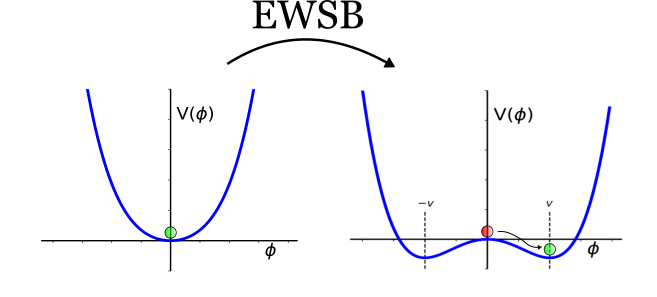
\includegraphics[width=0.75\textwidth]{figures/chapter1/higgs_potential_trans}
		\caption{Illustration of electroweak symmetry breaking (EWSB).
			\textbf{\textit{Left}}: Higgs potential with $\mu^2>0$ with stable equilibrium at $\phi=0$.
			\textbf{\textit{Right}}: With $\mu^2<0$, $\phi=0$ is no longer
			a stable equilibrium and the Higgs attains a non-zero vacuum
			expectation value at $\pm v$ --- breaking the \SUewk~gauge symmetry of the electroweak
			sector of the SM.
		}
	\label{fig:higgs_ewsb}
	\end{center}
\end{figure}

As opposed to `eating' gauge degrees of freedom as in the case of the \fieldWpm~and \fieldZ~bosons,
the fermion masses are obtained by adding additional interaction terms to \SML~between the
fermions and Higgs fields,
\begin{align}
	\mathcal{L}_{f-h} = y_f \left( \bar{L} \phi e^-_R + \phi^{\dagger} \overline{e^-}_R L\right).
	\label{eq:higgs_fermion_int}
\end{align}
Since both $L$ and $\phi$ are \SUtwo~doublets, adding the right-handed \SUtwo~singlet terms
do not spoil the \SUtwo~symmetry.
When the Higgs field acquires a non-zero vev after EWSB, we can insert Equation~\ref{eq:higgs_perturb} into Equation~\ref{eq:higgs_fermion_int} to obtain expressions for the fermions masses,
\begin{align}
	m_f = y_f \frac{v}{\sqrt{2}},
	\label{eq:fermion_mass_term}
\end{align}
where the $y_f$ are referred to as the fermion \textit{Yukawa couplings}, and are free parameters
of the SM that need to be measured.
Additional interactions arise between the fermions and $h(x)$ whose couplings are related
to the fermion masses as,
\begin{align}
	\mathcal{L}_{f-h} \propto \frac{m_f}{v} \bar{f}f h.
	\label{eq:higgs_fermion_coupling}
\end{align}

The general form Equation~\ref{eq:higgs_fermion_int} implies that the $y_f$ are matrices representing the
Higgs-fermion Yukawa couplings. They can be diagonalized by performing the proper unitary
transformations between the weak- and mass-bases of the fermion fields. In the case of the leptons,
this rotation is the identity: the lepton's weak eigenbasis is the same as their mass eigenbasis.
This is mainly due to the extraordinarily large mass difference between the charged and neutral
leptons within each lepton generation~\cite{Akhmedov:2007fk}. Within the quark-sector,  however,
the mass- and weak-basis fermion fields differ. This implies that the diagonalization procedure results
in mixing among the weak eigenstates of the quark fields to produce the observed mass eigenstates; i.e. the quark mass-eignstates ($d$,
$s$, $b$) are
coherent mixtures of the weak eigenstates ($d^{\prime}$,
$s^{\prime}$, $b^{\prime}$).\footnote{The mixing can be parametrised as either occurring between
the up-type, down-type, or a mixture of up- and down-type fields of each \SUtwo~doublet. Without
loss of generality and for simplicity, it is usually given with respect to the down-type quark fields as shown
here.}
This allows for the flavor-changing processes that are present
in charged weak interactions, allowing for interaction terms involving the decay
of a quark of one family into that of another family. The amount of mixing in the quark sector
is dictated by a $3\times 3$ unitary matrix known as the \textit{Cabibbo-Kobayashi-Maskawa} (CKM)
matrix~\cite{Kobayashi:1973fv} $\mathcal{V}_{\text{CKM}}$, the general form of which has four free parameters: three mixing angles
and a complex phase, $\delta$. The off-diagonal terms of the CKM matrix and the value of the mixing angles
dictate the amount of flavor mixing in the quark sector. The complex phase $\delta$
allows for charge-parity (CP) symmetry violating effects to occur. In fact, this term is the \textit{only} term of the SM
that allows for CP-violation --- an effect important for providing interactions that are asymmetric
between matter and anti-matter fields.\footnote{Charge Parity (CP) symmetry refers to the invariance
	of a theory with respect to swapping particles with their corresponding anti-particles and, additionally,
	inverting a field's spatial coordinates, $\psi(\vec{x}) \rightarrow \psi(-\vec{x})$. The former
	is the `C' symmetry and the latter is the `P' symmetry.
}

The remaining terms of $V(\phi)$ (Equation~\ref{eq:higgs_potential}) involve only the Higgs field. After
EWSB and the Higgs field acquiring vev we obtain,
\begin{align}
	V(\phi) \rightarrow V(\phi)_{\text{EWSB}} =  -\lambda \nu^2 h^2 - \lambda \nu h^3 - \frac{1}{4} \lambda h^4 + \text{const.}
	\label{eq:higgs_potential_self_int}
\end{align}
where we have ignored the terms already discussed above. The first term of Equation~\ref{eq:higgs_potential_self_int}
is the Higgs boson mass term, the second and third are the triple and quartic Higgs self-couplings,
\begin{align}
	\underbrace{m_{h} = \sqrt{ - 2 \mu^2} = \sqrt{ 2 \lambda v^2 }}_\text{Higgs boson mass} \hspace{1cm} \underbrace{\mathcal{L}_{hhh} \propto \frac{m_h^2}{v} \hspace{1cm} \mathcal{L}_{hhhh} \propto \frac{m_h^2}{v^2}}_\text{Triple and quartic Higgs self-couplings}.
	\label{eq:higgs_self_couplings}
\end{align}



